%%% demothesis.tex --- 
%% 
%% Filename: demothesis.tex
%% Description: 
%% Author: Ola Leifler
%% Maintainer: 
%% Created: Thu Oct 14 12:52:20 2010 (CEST)
%% Version: $Id$
%% Version: 
%% Last-Updated: Wed Jun 28 10:57:24 2017 (+0200)
%%           By: Ola Leifler
%%     Update #: 169
%% URL: 
%% Keywords: 
%% Compatibility: 
%% 
%%%%%%%%%%%%%%%%%%%%%%%%%%%%%%%%%%%%%%%%%%%%%%%%%%%%%%%%%%%%%%%%%%%%%%
%% 
%%% Commentary: 
%% 
%% 
%% 
%%%%%%%%%%%%%%%%%%%%%%%%%%%%%%%%%%%%%%%%%%%%%%%%%%%%%%%%%%%%%%%%%%%%%%
%% 
%%% Change log:
%% 
%% 
%% RCS $Log$
%%%%%%%%%%%%%%%%%%%%%%%%%%%%%%%%%%%%%%%%%%%%%%%%%%%%%%%%%%%%%%%%%%%%%%
%% 
%%% Code:

\documentclass[msc,lith,english]{liuthesis}
%% Settings go in settings.tex
%%% settings.tex --- 
%% 
%% Filename: settings.tex
%% Description: 
%% Author: Ola Leifler
%% Maintainer: 
%% Created: Tue Oct 19 21:11:31 2010 (CEST)
%% Version: $Id$
%% Version: 
%% Last-Updated: Tue Apr 25 08:49:48 2017 (+0200)
%%           By: Ola Leifler
%%     Update #: 43
%% URL: 
%% Keywords: 
%% Compatibility: 
%% 
%%%%%%%%%%%%%%%%%%%%%%%%%%%%%%%%%%%%%%%%%%%%%%%%%%%%%%%%%%%%%%%%%%%%%%
%% 
%%% Commentary: 
%% 
%% 
%% 
%%%%%%%%%%%%%%%%%%%%%%%%%%%%%%%%%%%%%%%%%%%%%%%%%%%%%%%%%%%%%%%%%%%%%%
%% 
%%% Change log:
%% 
%% 
%% RCS $Log$
%%%%%%%%%%%%%%%%%%%%%%%%%%%%%%%%%%%%%%%%%%%%%%%%%%%%%%%%%%%%%%%%%%%%%%
%% 
%%% Code:

\usepackage[backend=biber,hyperref]{biblatex}
%% To set the font of your thesis, use the \setmainfont{} command,
%% surrounded with \ifxetex if you want to switch between xelatex and pdflatex
\ifxetex 
%\setmainfont [Scale=1]{Georgia}
\fi

%%%%%%%%%%%%
%% The VZ43 chapter style, from Memoir contributed chapter styles: ftp://ftp.tex.ac.uk/ctan%3A/info/MemoirChapStyles/MemoirChapStyles.pdf
%%%%%%%%%%%

\usepackage{calc,color}
\newif\ifNoChapNumber
\newcommand\Vlines{%
\def\VL{\rule[-2cm]{1pt}{5cm}\hspace{1mm}\relax}
\VL\VL\VL\VL\VL\VL\VL}
\makeatletter
\setlength\midchapskip{0pt}
\makechapterstyle{VZ43}{
\renewcommand\chapternamenum{}
\renewcommand\printchaptername{}
\renewcommand\printchapternum{}

\renewcommand\chapnumfont{\Huge\bfseries\centering}
\renewcommand\chaptitlefont{\Huge\bfseries\raggedright}
\renewcommand\printchaptertitle[1]{%
\Vlines\hspace*{-2em}%
\begin{tabular}{@{}p{1cm} p{\textwidth-3cm}}%
\ifNoChapNumber\relax\else%
\colorbox{black}{\color{white}%
\makebox[.8cm]{\chapnumfont\strut \thechapter}}
\fi
& \chaptitlefont ##1
\end{tabular}
\NoChapNumberfalse
}
\renewcommand\printchapternonum{\NoChapNumbertrue}
}
\makeatother


%% To set bibliography options, refer to the biblatex manual and use
%% the ExecuteBibliographyOptions command below to set your options

\ExecuteBibliographyOptions{maxnames=99}


%% Change this to your appropriate BibTeX reference file (.bib)

\addbibresource{references.bib}

%%%%%%%%%%%%%%%%%%%%%%%%%%%%%%%%%%%%%%%%%%%%%%%%%%%%%%%%%%%%%%%%%%%%%%
%%% settings.tex ends here

%%% Local Variables: 
%%% mode: latex
%%% TeX-master: "demothesis"
%%% End: 

\usepackage{rotating}
\usepackage{eurosym}
\usepackage{color}
\usepackage{hyperref}
\usepackage[capitalize]{cleveref}
\usepackage{listings}
\usepackage{amssymb}
\usepackage{amsmath}
\usepackage{mathtools}
\usepackage{booktabs}
\usepackage{array}
%\usepackage[dvipsnames]{xcolor}
\usepackage{graphicx}
\usepackage{subcaption}

\newcolumntype{C}{>{$}c<{$}}

\graphicspath{{figures/}}

\definecolor{darkred}{rgb}{0.554, 0, 0}
\definecolor{darkblue}{rgb}{0, 0, 0.554}
\definecolor{darkgreen}{rgb}{0, 0.392, 0}
\definecolor{goldenrod}{rgb}{0.855, 0.647, 0.125}
\definecolor{cyan4}{RGB}{0, 139, 139}
\definecolor{turquoise}{RGB}{64, 224, 208}

\newenvironment{subs}
  {\adjustwidth{3em}{0pt}}
  {\endadjustwidth}

  \iffalse
  \lstdefinestyle{customc++}{
  classoffset=0,
  morekeywords={one,three,five},keywordstyle=\color{blue},
  classoffset=1,
  morekeywords={two,four,five},keywordstyle=\color{red},
  classoffset=0
  
%  basicstyle=\footnotesize\ttfamily,  
 % emph={float, int, vec3},
  %emphstyle={\color{darkred}},
  %stringstyle=\color{goldenrod},
  %captionpos=b,
%  numbers=left,
 % breaklines=true,
  %commentstyle=\itshape\color{darkgreen}
  }
  \fi

%\lstset{
 %   escapeinside={(*}{*)}
%}

% \usepackage{changebar}

%\newcommand{\norm}[1]{\lvert #1 \rvert}
%\newcommand{\dist}[1]{\lVert #1 \rVert}
\newcommand{\dist}[1]{\left\lVert #1 \right\rVert}

\DeclarePairedDelimiter{\norm}{\lVert}{\rVert}

\crefname{lstlisting}{listing}{listings}
\Crefname{lstlisting}{Listing}{Listings}

\department{Institutionen för Systemteknik}
\departmentenglish{Department of Electrical Engineering}
\departmentshort{ISY}

\externalsupervisor{Martin Olsson}
\supervisor{Harald Nautsch}
\examiner{Ingemar Ragnemalm}
\titleenglish{Evaluation of an Appearance\-Preserving Mesh Simplification Scheme for Configura AB}
\titleswedish{} 
\thesissubject{Computer Graphics and Visualization}

\publicationyear{2018}
\currentyearthesisnumber{001}
\dateofpublication{2018-01-01}

\author{Rasmus Hedin}

\hbadness=10000

\begin{document}

\chapterstyle{VZ43}

%%% Intro.tex --- 
%% 
%% Filename: Intro.tex
%% Description: 
%% Author: Ola Leifler
%% Maintainer: 
%% Created: Thu Oct 14 12:54:47 2010 (CEST)
%% Version: $Id$
%% Version: 
%% Last-Updated: Thu May 19 14:12:31 2016 (+0200)
%%           By: Ola Leifler
%%     Update #: 5
%% URL: 
%% Keywords: 
%% Compatibility: 
%% 
%%%%%%%%%%%%%%%%%%%%%%%%%%%%%%%%%%%%%%%%%%%%%%%%%%%%%%%%%%%%%%%%%%%%%%
%% 
%%% Commentary: 
%% 
%% 
%% 
%%%%%%%%%%%%%%%%%%%%%%%%%%%%%%%%%%%%%%%%%%%%%%%%%%%%%%%%%%%%%%%%%%%%%%
%% 
%%% Change log:
%% 
%% 
%% RCS $Log$
%%%%%%%%%%%%%%%%%%%%%%%%%%%%%%%%%%%%%%%%%%%%%%%%%%%%%%%%%%%%%%%%%%%%%%
%% 
%%% Code:


\chapter{Introduction}
\label{cha:introduction}

The introduction shall be divided into these sections:

\section{Motivation}
\label{sec:motivation}

This is where the studied problem is described from a general
point of view and put in a context which makes it clear that
it is interesting and well worth studying. The aim is to make
the reader interested in the work and create an urge to
continue reading.

\section{Aim}
\label{sec:aim}

What is the underlying purpose of the thesis project?

\section{Research questions}
\label{sec:research-questions}


This is where the research questions are described.
Formulate these as explicit questions, terminated with a
question mark. A report will usually contain several different
research questions that are somehow thematically connected.
There are usually 2-4 questions in total.

Examples of common types of research questions (simplified
and generalized):

\begin{enumerate}
\item How does technique X affect the possibility of achieving the
  effect Y?

\item How can a system (or a solution) for X be realized so
  that the effect Y is achieved?

\item What are the alternatives to
  achieving X, and which alternative gives the best effect considering
  Y and Z? (This research question is normally broken down in to 2
  separate questions.)

\end{enumerate}


Observe that a very specific research question almost always
leads to a better thesis report than a general research question
(it is simply much more difficult to make something good
from a general research question.)

The best way to achieve a really good and specific research
question is to conduct a thorough literature review and get
familiarized with related research and practice. This leads to
ideas and terminology which allows one to express oneself
with precision and also have something valuable to say in the
discussion chapter. And once a detailed research question
has been specified, it is much easier to establish a suitable
method and thus carry out the actual thesis work much faster
than when starting with a fairly general research question. In
the end, it usually pays off to spend some extra time in the
beginning working on the literature review. The thesis
supervisor can be of assistance in deciding when the research
question is sufficiently specific and well-grounded in related
research.

\section{Delimitations}
\label{sec:delimitations}

This is where the main delimitations are described. For
example, this could be that one has focused the study on a
specific application domain or target user group. In the
normal case, the delimitations need not be justified.

%\nocite{scigen}
%We have included Paper \ref{art:scigen}

%%%%%%%%%%%%%%%%%%%%%%%%%%%%%%%%%%%%%%%%%%%%%%%%%%%%%%%%%%%%%%%%%%%%%%
%%% Intro.tex ends here


%%% Local Variables: 
%%% mode: latex
%%% TeX-master: "demothesis"
%%% End: 

%%% lorem.tex --- 
%% 
%% Filename: lorem.tex
%% Description: 
%% Author: Ola Leifler
%% Maintainer: 
%% Created: Wed Nov 10 09:59:23 2010 (CET)
%% Version: $Id$
%% Version: 
%% Last-Updated: Tue Oct  4 11:58:17 2016 (+0200)
%%           By: Ola Leifler
%%     Update #: 7
%% URL: 
%% Keywords: 
%% Compatibility: 
%% 
%%%%%%%%%%%%%%%%%%%%%%%%%%%%%%%%%%%%%%%%%%%%%%%%%%%%%%%%%%%%%%%%%%%%%%
%% 
%%% Commentary: 
%% 
%% 
%% 
%%%%%%%%%%%%%%%%%%%%%%%%%%%%%%%%%%%%%%%%%%%%%%%%%%%%%%%%%%%%%%%%%%%%%%
%% 
%%% Change log:
%% 
%% 
%% RCS $Log$
%%%%%%%%%%%%%%%%%%%%%%%%%%%%%%%%%%%%%%%%%%%%%%%%%%%%%%%%%%%%%%%%%%%%%%
%% 
%%% Code:

\chapter{Theory} \label{ch:theory}

\section{Mesh Simplification} \label{sec:mesh_simplification}

\subsection{Quadric-Based Error Metrics} \label{sec:quadric-based_error_metrics}

\subsection{Appearance-Preserving Simplification} \label{sec:appearance-preserving_simplification}

\subsection{Texture Mapped Progressive Meshes} \label{sec:texture-mapped_progressive_meshes}
Given an arbitrary mesh, Hoppe et. al \cite{hoppe1996progressive} presents a method to construct a \emph{progressive mesh} (PM) where a texture parametrization is shared between all meshes in a PM sequence. In order to create a texture mapping for a simplified mesh, the original mesh's attributes, e.g normals, is sampled. This method was developed with two goals taken into consideration:
\begin{itemize}
\item{Minimize \emph{texture stretch}:}~~~When a mesh is simplified the texture may be stretched in some areas which decrease the quality of the appearance. Since the texture parametrization determines the sampling density, a balanced parametrization is prefered over one that samples with different density in different areas. The balanced parametrization is obtained by minimizing the largest texture stretch over all points in the domain. No point in the domain will therefore not be too stretched and thus making no point undersampled. 
\item{Minimize \emph{texture deviation}:}~~~Conventional methods use geometric error for the mesh simplification. According to the authors this is not appropriate when a mesh is textured. The stricter texture deviation error metric, where the geometric error is measured according to the parametrization, is more appropriate. By plotting a graph of the texture deviation vs the number of faces, the goal is to minimize the heighf of this graph.
\end{itemize}


\section{Metrics for Appearance Preservation} \label{sec:metrics_for_appearance_preservation}

\section{Measuring Performance} \label{measuring_performance}

%%%%%%%%%%%%%%%%%%%%%%%%%%%%%%%%%%%%%%%%%%%%%%%%%%%%%%%%%%%%%%%%%%%%%%
%%% theory.tex ends here

%%% Local Variables: 
%%% mode: latex
%%% TeX-master: "thesis"
%%% End: 

%%% lorem.tex --- 
%% 
%% Filename: lorem.tex
%% Description: 
%% Author: Ola Leifler
%% Maintainer: 
%% Created: Wed Nov 10 09:59:23 2010 (CET)
%% Version: $Id$
%% Version: 
%% Last-Updated: Wed Nov 10 09:59:47 2010 (CET)
%%           By: Ola Leifler
%%     Update #: 2
%% URL: 
%% Keywords: 
%% Compatibility: 
%% 
%%%%%%%%%%%%%%%%%%%%%%%%%%%%%%%%%%%%%%%%%%%%%%%%%%%%%%%%%%%%%%%%%%%%%%
%% 
%%% Commentary: 
%% 
%% 
%% 
%%%%%%%%%%%%%%%%%%%%%%%%%%%%%%%%%%%%%%%%%%%%%%%%%%%%%%%%%%%%%%%%%%%%%%
%% 
%%% Change log:
%% 
%% 
%% RCS $Log$
%%%%%%%%%%%%%%%%%%%%%%%%%%%%%%%%%%%%%%%%%%%%%%%%%%%%%%%%%%%%%%%%%%%%%%
%% 
%%% Code:

\chapter{Method}
\label{cha:method}

In this chapter, the method is described in a way which shows how the
work was actually carried out. The description must be precise and
well thought through. Consider the scientific term
replicability. Replicability means that someone reading a scientific
report should be able to follow the method description and then carry
out the same study and check whether the results obtained are
similar. Achieving replicability is not always relevant, but precision
and clarity is.

Sometimes the work is separated into different parts, e.g.  pre-study,
implementation and evaluation. In such cases it is recommended that
the method chapter is structured accordingly with suitable named
sub-headings.

%%%%%%%%%%%%%%%%%%%%%%%%%%%%%%%%%%%%%%%%%%%%%%%%%%%%%%%%%%%%%%%%%%%%%%
%%% lorem.tex ends here

%%% Local Variables: 
%%% mode: latex
%%% TeX-master: "demothesis"
%%% End: 

%%%%%%%%%%%%%%%%%%%%%%%%%%%%%%%%%
%  Figure subfigure template
%%%%%%%%%%%%%%%%%%%%%%%%%%%%%%%%%
\iffalse

\begin{figure}[ht]
  \centering
  \begin{subfigure}[b]{\textwidth}
    \centering
    \includegraphics[width=\textwidth]{}
    \caption{}
    \label{}
  \end{subfigure}
  \caption{}
  \label
\end{figure}

\fi



\chapter{Results} \label{cha:results}
In this chapter the results of the thesis is presented. First, results collected using multiple metrics for mesh appearance are presented. Afterwards, a comparison of the execution time using different numbers of threads is given. Finally, simplified models generated to be used as LoD:s as well as the new improved texture atlas is presented.

\section{Luminance error}

RMS luminance error was computed by rendering multiple images of a model from different camera positions as explained in \cref{sec:metrics_for_appearance_preservation} and can be seen in \cref{fig:mean_luminance_error}. Four LoD:s are presented where \emph{super} have the most amount of triangles and \emph{low} have the least amount of triangles. The error was measured for different settings of seam and volume preservation to determine what setting would give the best result. Nine different models with triangle counts between 10000 and 30118 was used in this evaluation. For each model the RMS luminance error was computed for all LoD:s. A mean of the RMS was then obtained and is presented together with a 95\% confidence interval in \cref{fig:mean_luminance_error}.

\begin{figure}[h]
  \centering
  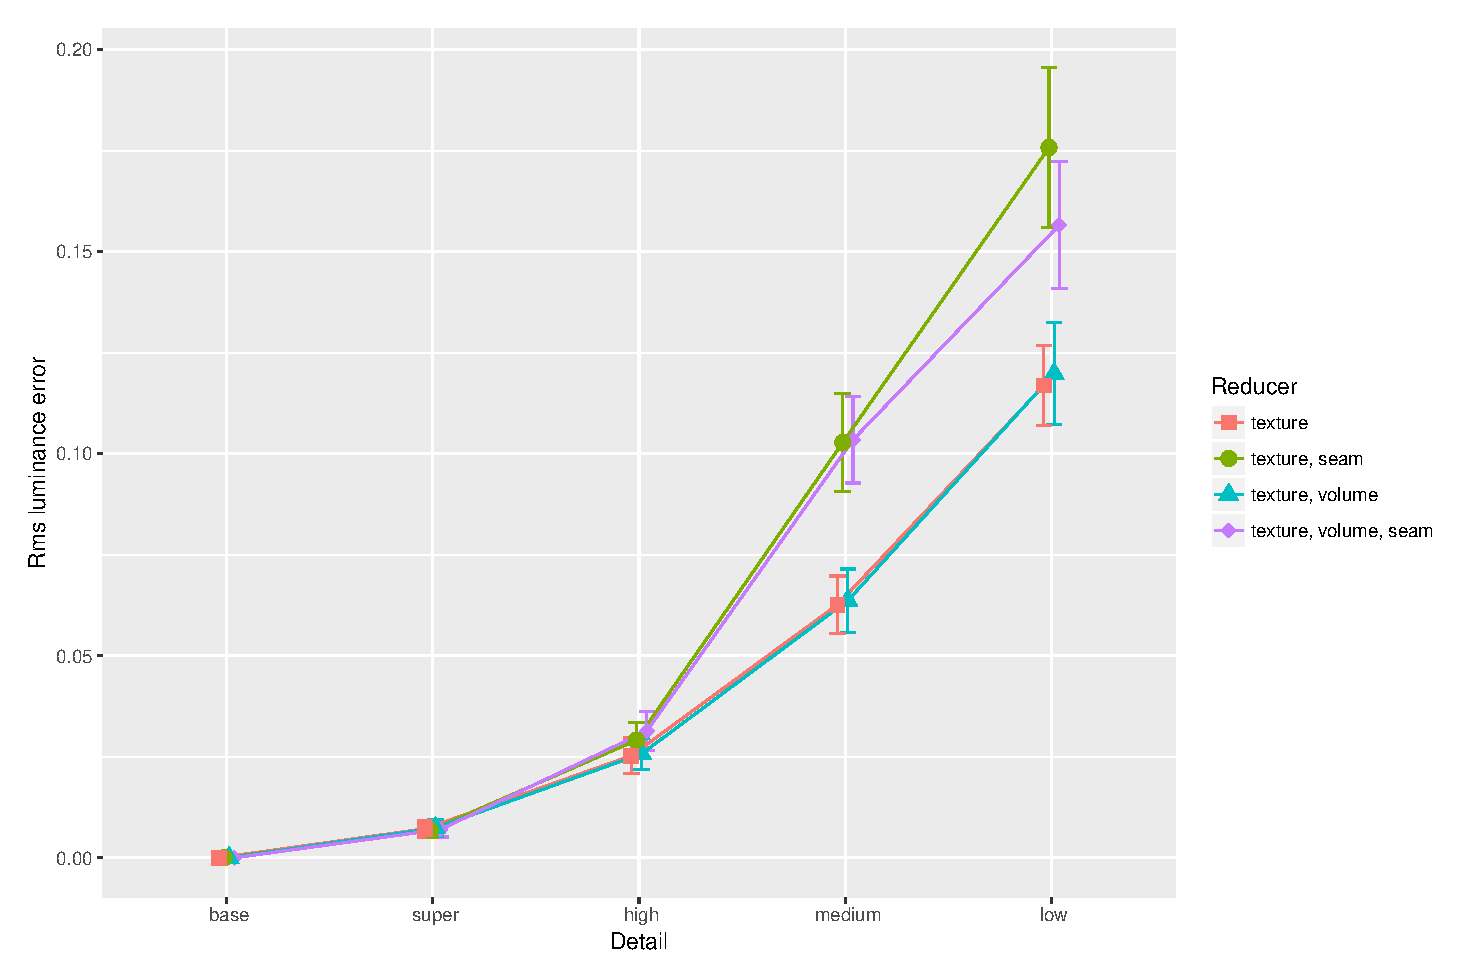
\includegraphics[width=.55\textwidth]{Rdata/rms_luminance.eps}
  \caption{Rms luminance error}
  \label{fig:mean_luminance_error}
\end{figure}

\clearpage

\section{Geometric and Color Error}
To see how the geometry and color of a model is affected by simplification, points were sampled on the surface of the simplified mesh and the original mesh. The distances from the sampled points on one mesh to the closest points on the other mesh can then be used to measure the distance between the meshes as well as the color difference. This is described in more detail in \cref{sec:evaluation}. Both the RMS and the maximum error was measured for different settings of seam and volume preservation with the \emph{office woman model} and the values are plotted in \cref{fig:geo_col_error}. Note that the x-axis and y-axis have a logarithmic scale.

\begin{figure}[ht]
  \centering
  \begin{subfigure}[b]{.49\textwidth}
    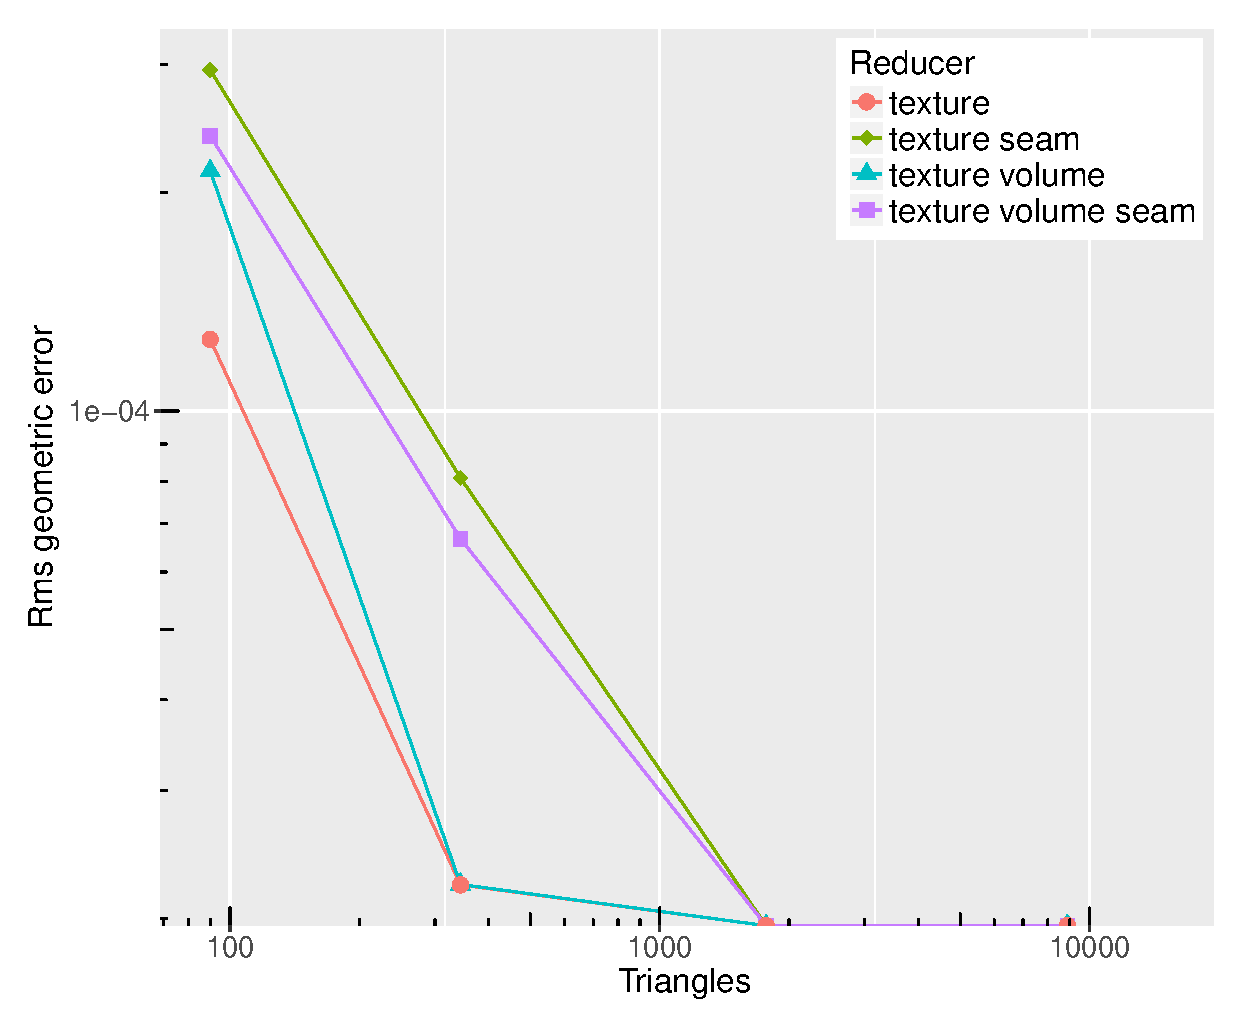
\includegraphics[width=\textwidth]{Rdata/rms_geometric_800.eps}
  \end{subfigure}
  \hfill
  \begin{subfigure}[b]{.49\textwidth}
    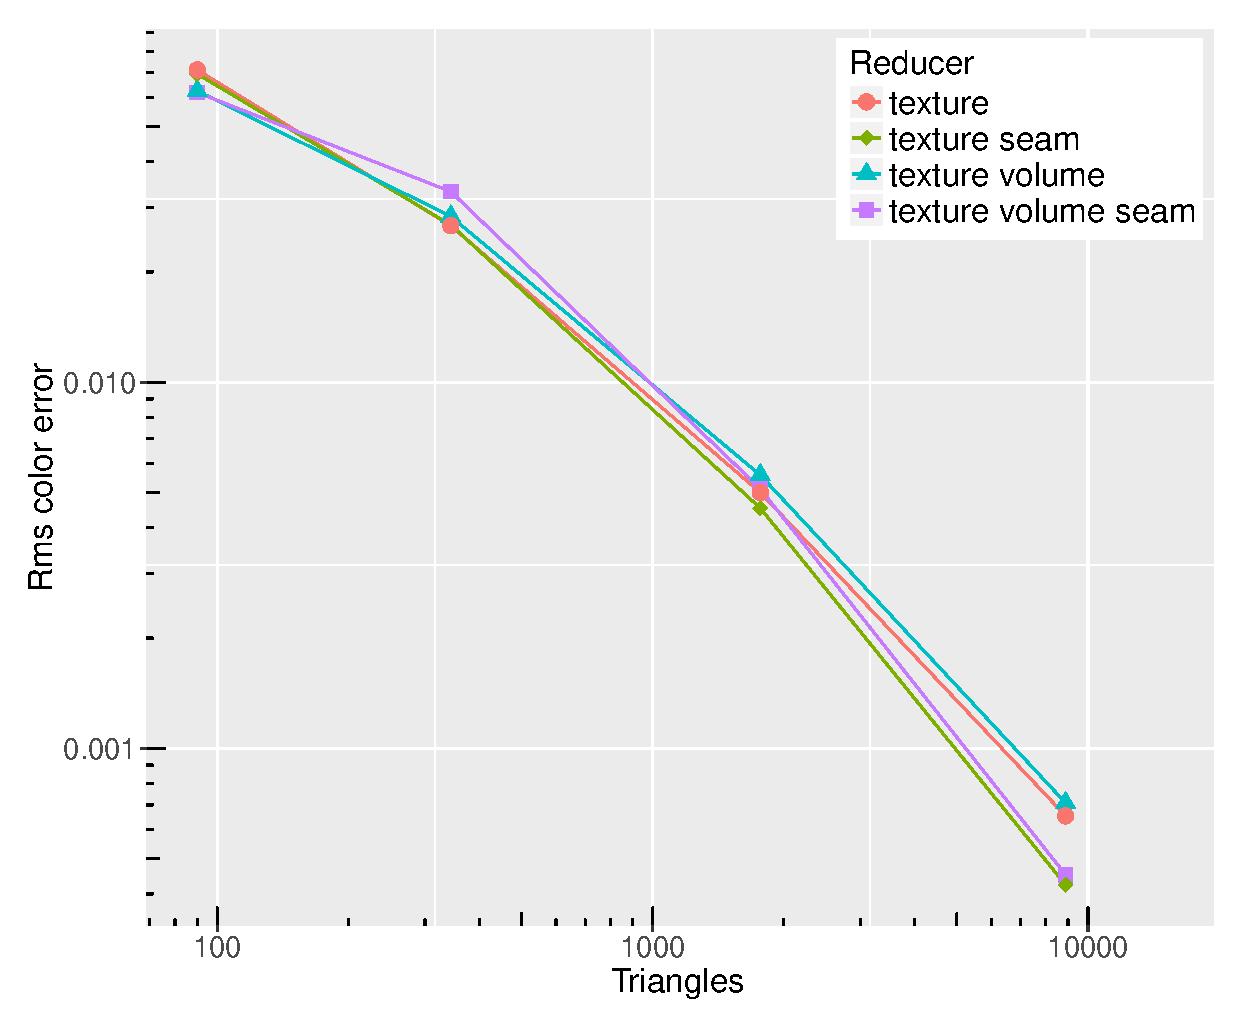
\includegraphics[width=\textwidth]{Rdata/rms_color_800.eps}
  \end{subfigure}

  \begin{subfigure}[b]{.49\textwidth}
    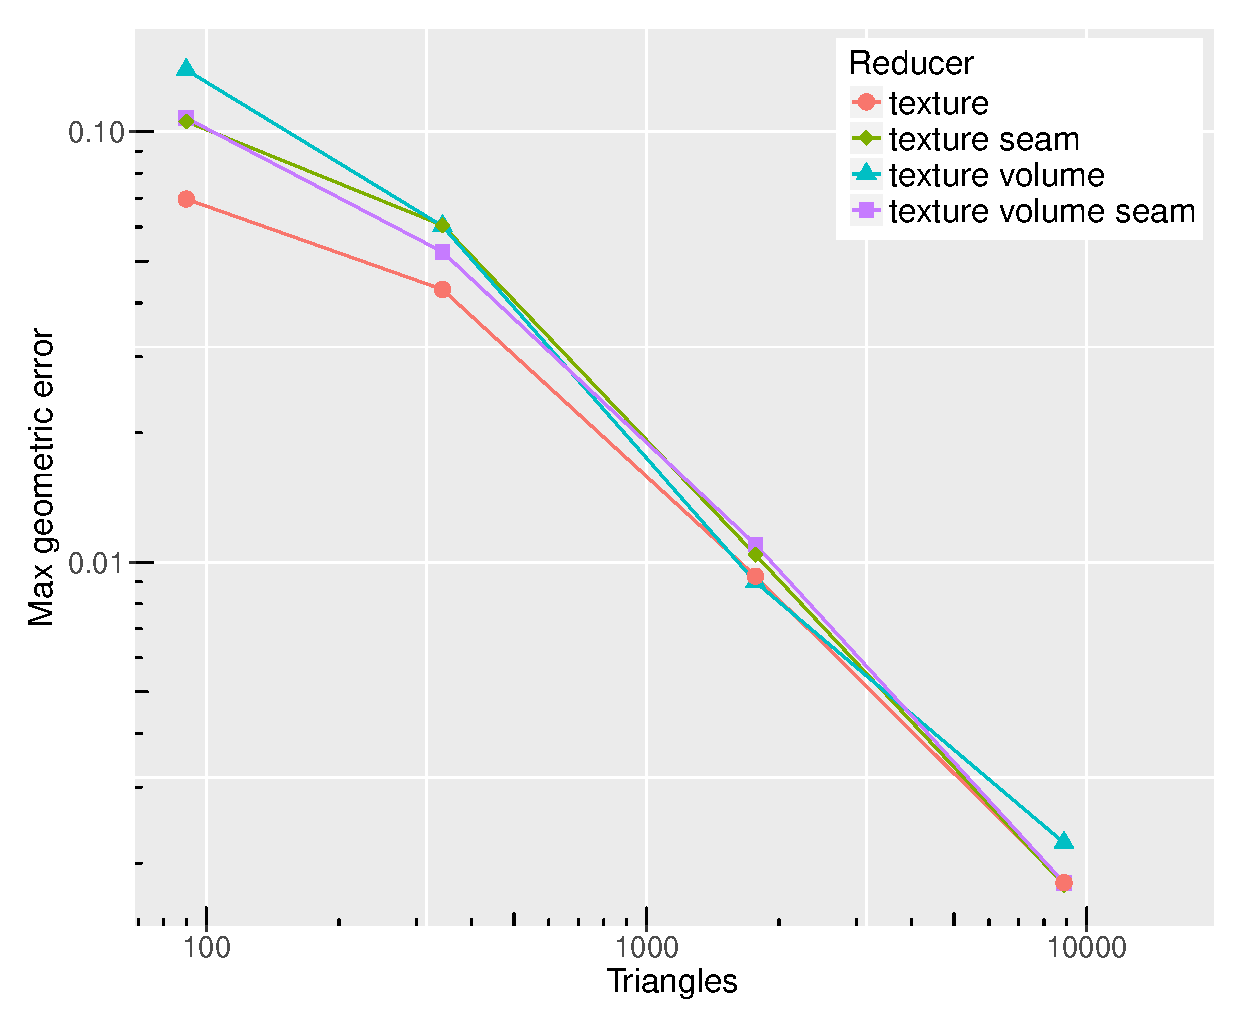
\includegraphics[width=\textwidth]{Rdata/max_geometric_800.eps}
  \end{subfigure}
  \hfill
  \begin{subfigure}[b]{.49\textwidth}
    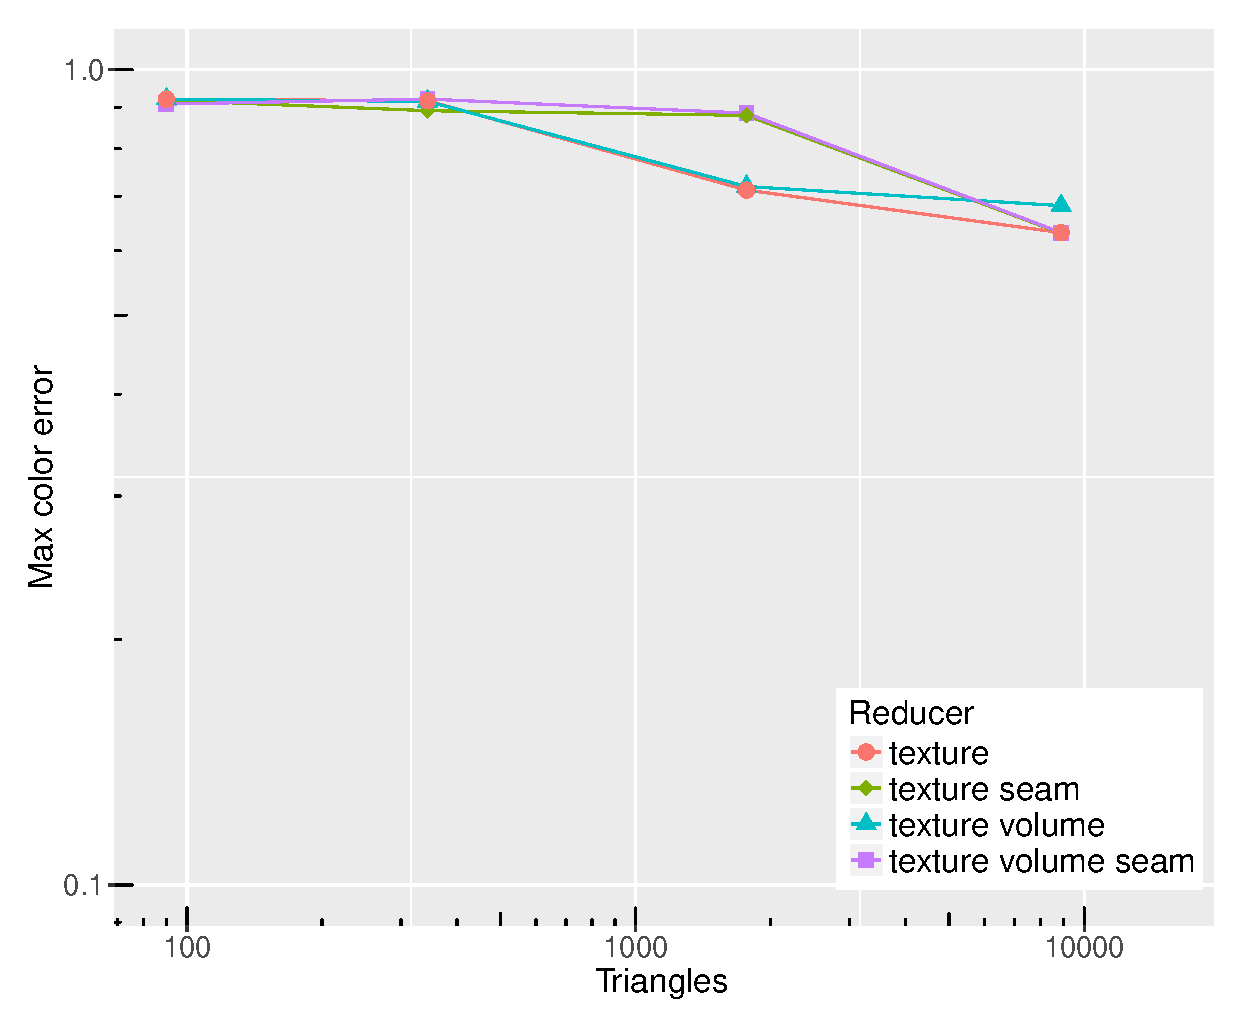
\includegraphics[width=\textwidth]{Rdata/max_color_800.eps}
  \end{subfigure}
  \caption{Office woman geometric and color error}
  \label{fig:geo_col_error}
\end{figure}

\clearpage
        
\section{Volume Preservation}
When simplification is performed the volume of the mesh may be reduced. How much the volume of a simplified mesh differ from the original mesh is therefore plotted in \cref{fig:volume_diff}. Reduction was made with four configurations of texture, volume, and seam considerations for nine models. The mean difference in volume is plotted together with a 95\% confidence interval.

\begin{figure}[ht]
  \centering
  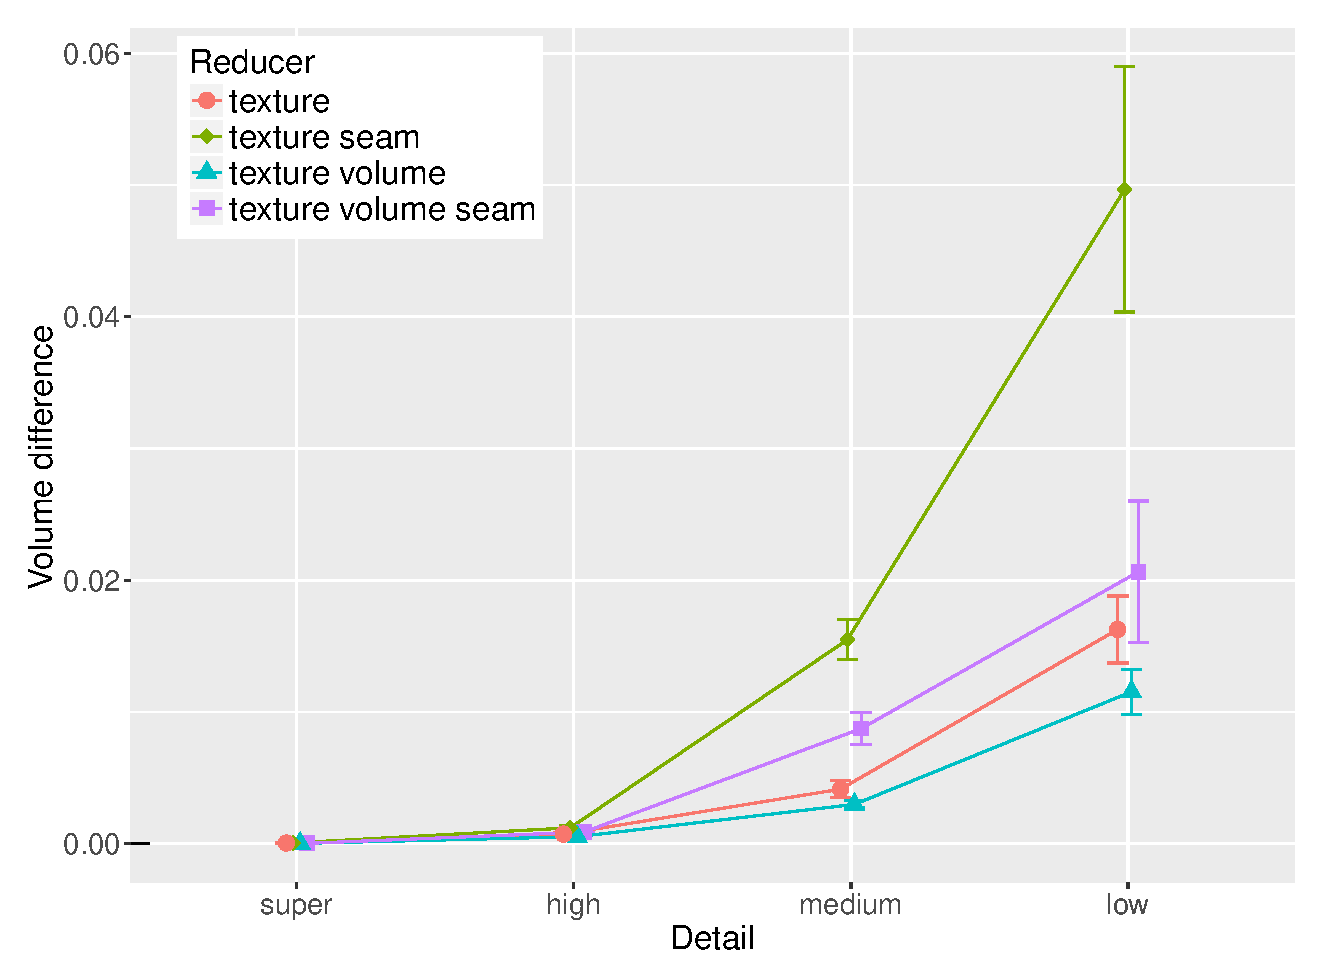
\includegraphics[width=\textwidth]{Rdata/volume_diff.eps}
  \caption{Mean difference in volume}
  \label{fig:volume_diff}
\end{figure}

\clearpage

\section{Execution time}
Four LoD:s were generated with the mesh simplification scheme multiple times. The mean execution time in milliseconds for different number of threads running in parallel is plotted in \cref{fig:execution_time} with a 95\% confidence interval.

\begin{figure}[ht]
  \centering
  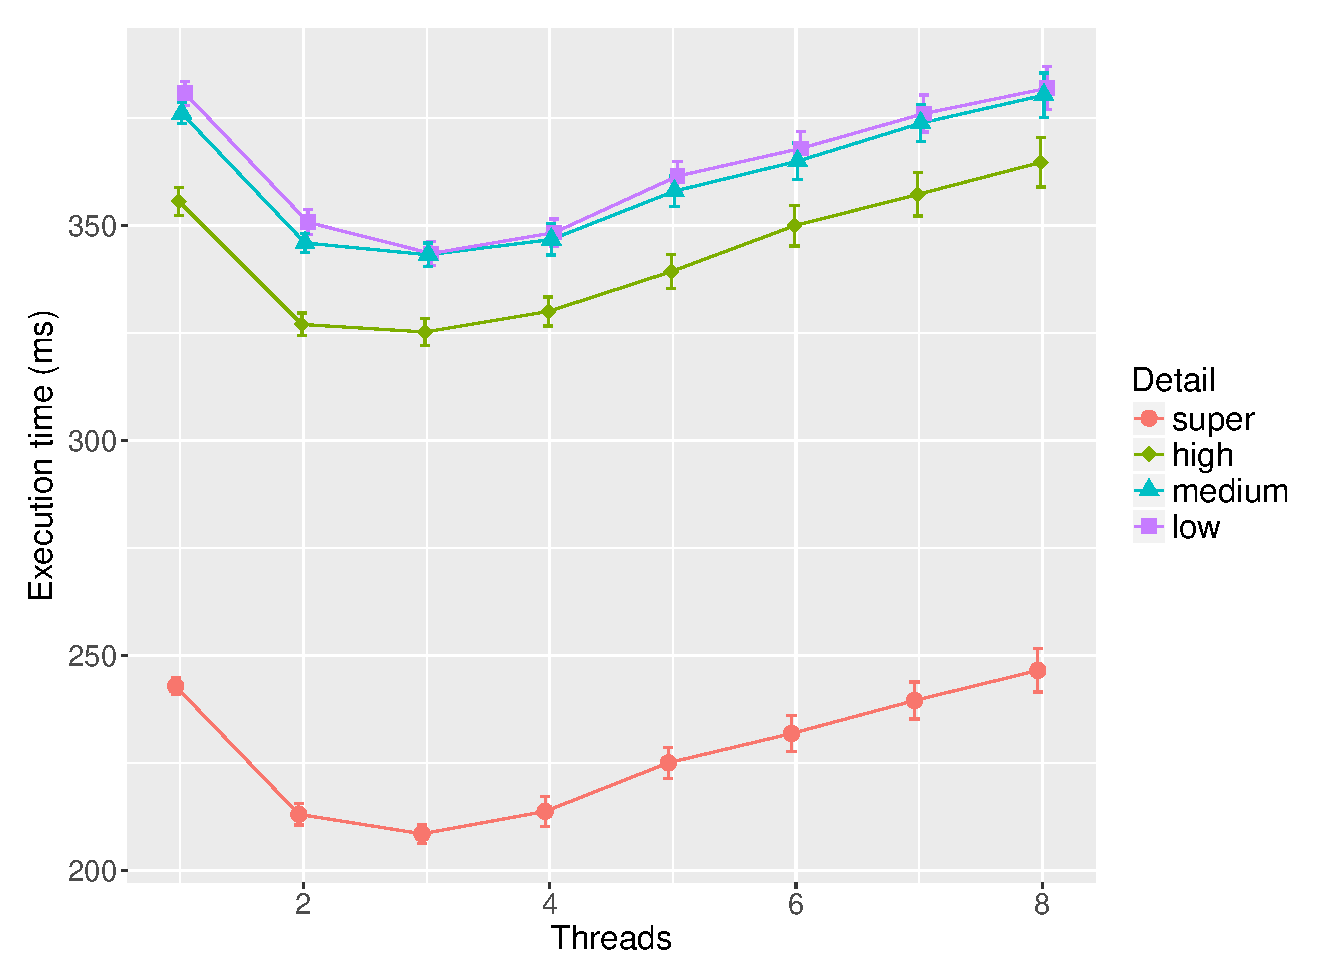
\includegraphics[width=\textwidth]{Rdata/parallel_execution_time.eps}
  \caption{Mean execution time when using multiple threads}
  \label{fig:execution_time}
\end{figure}

\clearpage

\section{Improved Texture Atlas}
A pull-push algorithm was implemented in order to improve the texture that is used by a mesh since undefined areas may be seen when applied to a simplified model. Given a texture (\cref{fig:original_texture_atlas}), rays are casted for each pixel in order to generate a black and white image that distinguish valid pixels from invalid pixels. Valid pixels get a white color and invalid pixels a black color as seen in \cref{fig:valid_pixels}. Pixels with a corresponding black pixel will be filled in by the pull-push algorithm. This will result in the texture seen in \cref{fig:improved_texture} where all the empty pixels have been filled in.

\begin{figure}[ht]
  \centering
  \begin{subfigure}[b]{.3\textwidth} 
    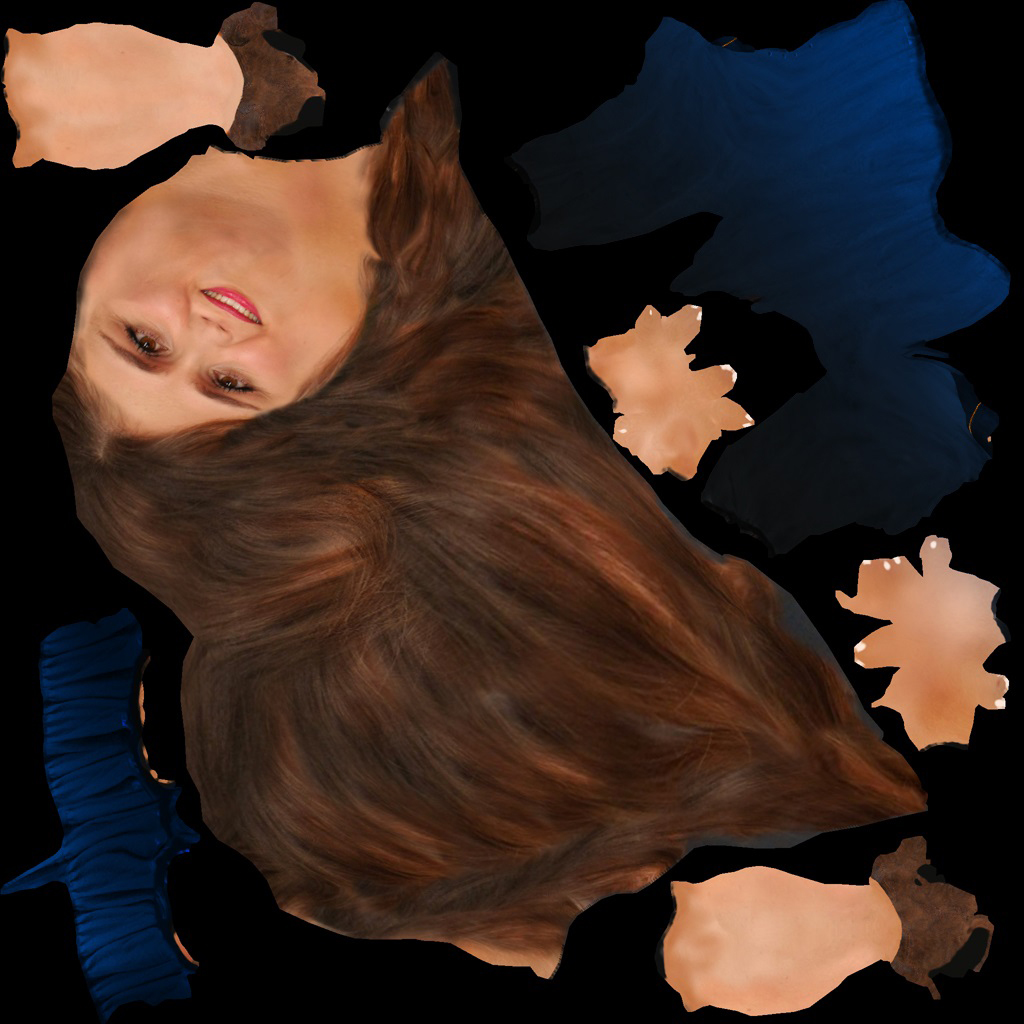
\includegraphics[width=\textwidth]{woman_input.jpg}
    \caption{Original}
    \label{fig:original_texture_atlas}
  \end{subfigure}
  ~
  \begin{subfigure}[b]{.3\textwidth}
    
\includegraphics[width=\textwidth]{woman_bound.png}
    \caption{Valid pixels}
    \label{fig:valid_pixels}
  \end{subfigure}
  ~
  \begin{subfigure}[b]{.3\textwidth}
    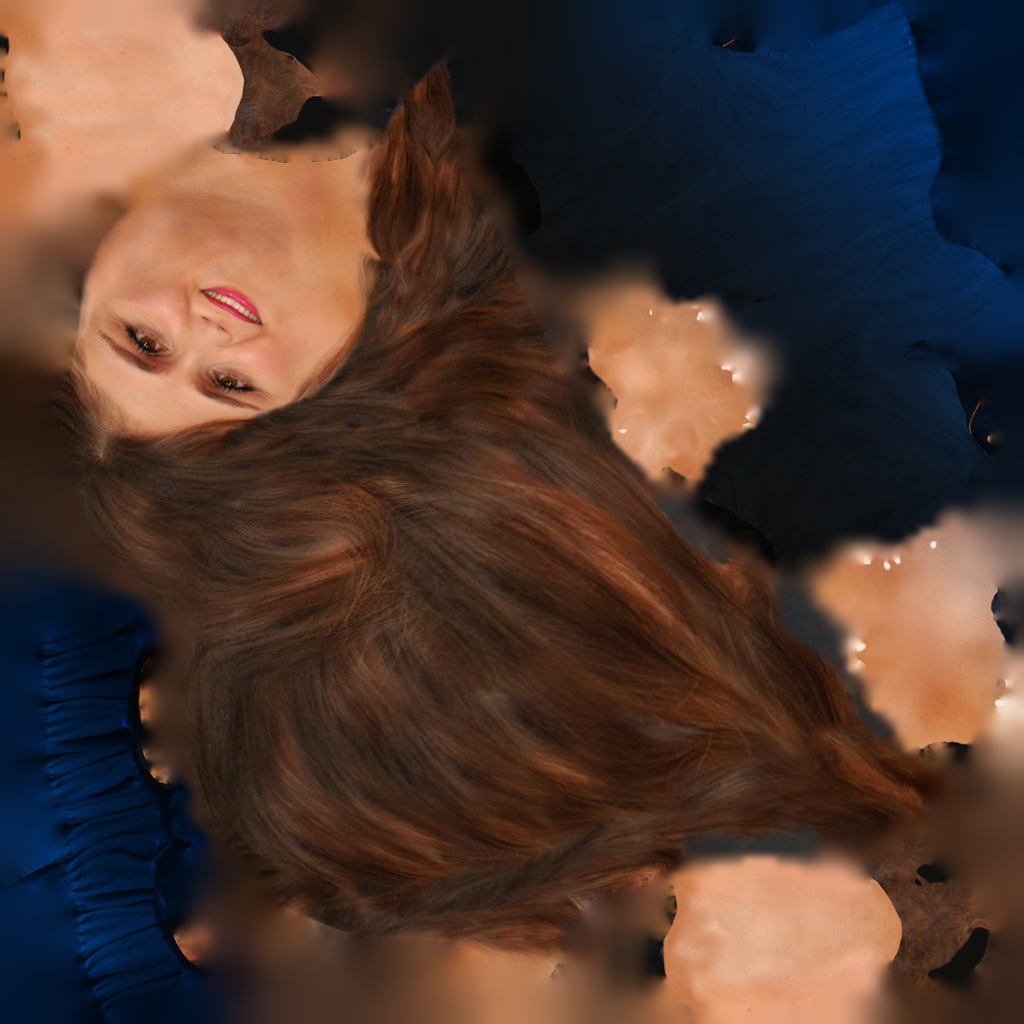
\includegraphics[width=\textwidth]{woman_output.png}
    \caption{Improved texture}
    \label{fig:improved_texture}
  \end{subfigure}
  \caption{Filling in empty pixels in the texture atlas}
  \label{fig:improve_texture_atlas}
\end{figure}

Simplification of the office woman model introduced black areas on the legs where the original seam used to be (\cref{fig:using_original_texture}). Trying to improve the appearance by applying the new improved texture results in the model shown in \cref{fig:using_improved_texture}.

\begin{figure}[ht]
  \centering
  \begin{subfigure}[b]{.15\textwidth}
    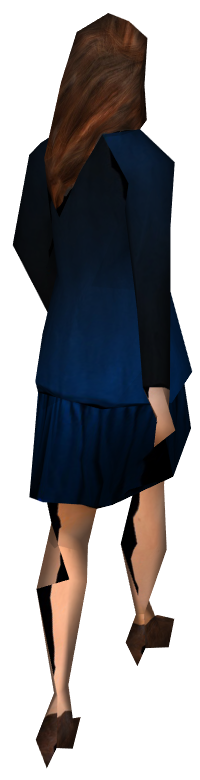
\includegraphics[width=\textwidth]{woman_render.png}
    \caption{Using original texture}
    \label{fig:using_original_texture}
  \end{subfigure}
  \qquad
  \begin{subfigure}[b]{.15\textwidth}
    
\includegraphics[width=\textwidth]{woman_render_improved.png}
    \caption{Using improved texture}
    \label{fig:using_improved_texture}
  \end{subfigure}
  \caption{Comparison between original and improved texture}
  \label{fig:texture_comparison}
\end{figure}

\clearpage

% base:   14996
% super:   8886
% high:    1768
% medium:   344
% low:       90
\section{Comparison of LoD:s}

To compare how different LoD:s are affected by the simplification the office woman model have been rendered after simplification. The original model has 14996 triangles and the LoD:s super, high, medium, and low have 8886, 1768, 344, 90 triangles respectively. Renderings of the Lod:s have been created both with equal distance from the camera and with the camera placed at the distance where they would actually be used which can be seen in \cref{fig:woman_lodeq,fig:woman_lod} respectively. When creating these LoD:s with the simplification algorithm the seam and volume was not considered, only the texture.

\begin{figure}[ht]
  \centering
  \begin{subfigure}[b]{.22\textwidth}
    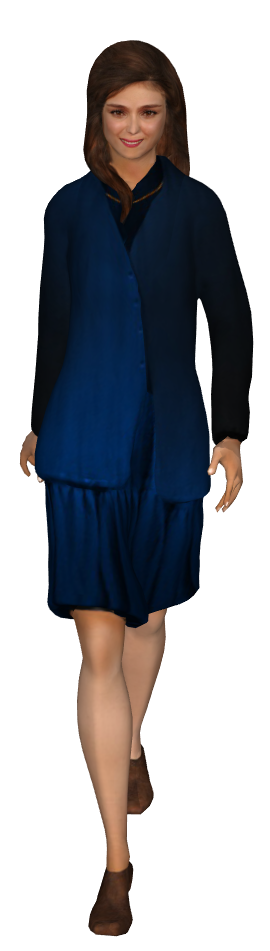
\includegraphics[width=\textwidth]{woman/equal_distance/1.png}
    \caption{super}
    \label{fig:womaneq0}
  \end{subfigure}
  \begin{subfigure}[b]{.22\textwidth}
    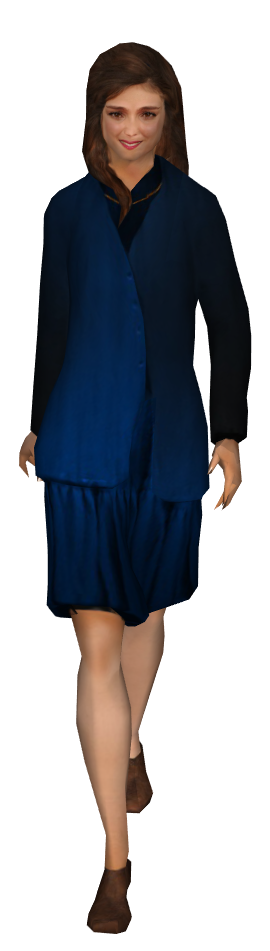
\includegraphics[width=\textwidth]{woman/equal_distance/2.png}
    \caption{high}
    \label{fig:womaneq1}
  \end{subfigure}
  \centering
  \begin{subfigure}[b]{.22\textwidth}
    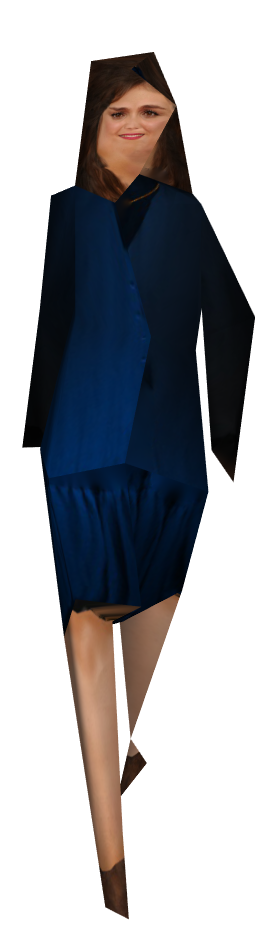
\includegraphics[width=\textwidth]{woman/equal_distance/3.png}
    \caption{medium}
    \label{fig:womaneq2}
  \end{subfigure}
  \begin{subfigure}[b]{.22\textwidth}
    
\includegraphics[width=\textwidth]{woman/equal_distance/4.png}
    \caption{low}
    \label{fig:womaneq3}
  \end{subfigure}
  \caption{Office woman LoD:s at equal distance}
  \label{fig:woman_lodeq}
\end{figure}

\begin{figure}[ht]
  \centering
  \begin{subfigure}[b]{.22\textwidth}
    
\includegraphics[width=\textwidth]{woman/cropped/1.png}
    \caption{super}
    \label{fig:woman0}
  \end{subfigure}
  \begin{subfigure}[b]{.22\textwidth}
    
\includegraphics[width=\textwidth]{woman/cropped/2.png}
    \caption{high}
    \label{fig:woman1}
  \end{subfigure}
  \centering
  \begin{subfigure}[b]{.22\textwidth}
    
\includegraphics[width=\textwidth]{woman/cropped/3.png} 
    \caption{medium}
    \label{fig:woman2}
  \end{subfigure}
  \begin{subfigure}[b]{.22\textwidth}
    
\includegraphics[width=\textwidth]{woman/cropped/4.png}
    \caption{low}
    \label{fig:woman3}
  \end{subfigure}
  \caption{Office woman LoD:s at their corresponding distance} 
  \label{fig:woman_lod}
\end{figure}

%%% discussion.tex --- 
%% 
%% Filename: discussion.tex
%% Description:
%% Author:
%% Maintainer: 
%% Created:
%% Version:
%% Version:
%% Last-Updated:
%%           By:
%%     Update #:
%% URL: 
%% Keywords: 
%% Compatibility: 
%% 
%%%%%%%%%%%%%%%%%%%%%%%%%%%%%%%%%%%%%%%%%%%%%%%%%%%%%%%%%%%%%%%%%%%%%%
%% 
%%% Commentary: 
%% 
%% 
%% 
%%%%%%%%%%%%%%%%%%%%%%%%%%%%%%%%%%%%%%%%%%%%%%%%%%%%%%%%%%%%%%%%%%%%%%
%% 
%%% Change log:
%% 
%% 
%% RCS $Log$
%%%%%%%%%%%%%%%%%%%%%%%%%%%%%%%%%%%%%%%%%%%%%%%%%%%%%%%%%%%%%%%%%%%%%%
%% 
%%% Code:

\chapter{Discussion} \label{cha:discussion}
This chapter provides a discussion on the work. First, a discussion of the results is given in \cref{sec:discussion_result}. Afterwards, in \cref{sec:discussion_method} the used method is discussed.

\section{Result} \label{sec:discussion_result}


\subsection{Luminance Error} \label{sec:discussion_luminance}
When simplifying a mesh to be used for LoD super and high, considering the seam or the volume does not affect the rms luminance error much as can be seen in \cref{fig:mean_luminance_error}. At the high level the graphs start to diverge but the confidence intervals overlap which means that we can not say with any significance that any setting is better than another. However, for medium and low, considering the seam gives a worse result than not considering it.

Not allowing all edge removals in the seam constrains the simplification and this affects the final geometry. Geometry that differs a lot from the original will give a high luminance error. This occurs since in some areas of the rendered images the background is rendered where the mesh used to be. In this case the background was white leading to a high difference of the images.

Ignoring the seam for now, if the volume is considered the error becomes slightly larger but not with any significance. Not considering the volume may be a better choice since the optimization problem would be less constrained and could be solved faster.

\subsection{Color and Geometric Error} \label{sec:discussion_color_geom}
To further investigate when the seam and volume should be considered points was sampled on the surfaces of the mesh. A comparison of this can be seen in \cref{fig:geo_col_error}.

If we first look at the geometric error the two highest LoD:s have a geometric error close to zero for all settings. For the other two lower levels we can see, just as discussed in \cref{sec:discussion_luminance}, that the seam preservation give a worse result. According the graphs of the geometric error the best setting would be to only consider the texture.

When looking at the color error the difference is small between the settings. However, the rms color error for the super LoD is lower when the seam is considered. Therefore, considering the seam may give a better result for the super and high LoD since the geometric error was small.

\subsection{Volume Preservation} \label{sec:discussion_volume}
\cref{fig:volume_diff} shows how the volume of meshes is affected by different configurations of texture, seam and volume preservation. Just as discussed in previous sections the configuration affect the result for the two highest LoD:s very little. By looking at the figure we can see that the volume constraint indeed keep the volume better. Considering the seam gives a larger difference in volume but it is kept better if the volume is also consider. The best configuration if one wants to keep the volume is to only consider the texture and the volume.

\subsection{Execution Time} \label{sec:discussion_time}
By looking at \cref{fig:execution_time} we can see the difference when using multiple threads. Parallelization was only added to the initialization phase of the simplification since it did not have that many dependent operations. A gain in speed can be noticed by just using one more thread. The total execution time is only decreased by about 30 ms which is only a decrease of 12\%.

For all four LoD:s the curves are similar. The similarity is expected since the same initial computations is performed for all levels and no parallelization is performed during the simplification phase.

The fastest execution time is obtained when using between 2 to 4 threads. Using more threads seem to increase the execution time. This could be because the threads have to wait for each other to write to the quadric matrices. In the implementation only one thread at a time can write which is not desirable.


\subsection{Improved Texture Atlas} \label{sec:discussion_texture}
As we have seen from the graphs the seam gives a bad result in terms of luminance error and geometric error. But, when the seam is not considered undefined areas of the texture may appear just at the seam. This can be seen in \cref{fig:using_original_texture} where where black areas have appeared on the legs of the model.

Using the pull-push algorithm to fill in missing pixel values results in a new texture that gives a better result in the seams. As can be seen in \cref{fig:using_improved_texture} almost all the black areas have disappeared from the legs. However, on the left leg a small hint of black can be seen. By looking at the new texture we can see that there still remains some black areas just at the seam bound.


\subsection{Comparison of LoD:s} \label{sec:discussion_lod}
Looking at the four LoD:s of the office woman model in \cref{fig:woman_lodeq} we can see how the different levels are affected by simplification. The super and high have not changed very much the the appearance is still good. One can see that the silhouette of the high LoD is not as round as the super LoD. For medium the effect of the simplification is clear and even more for the low LoD where we can clearly see the triangles.

When looking at the LoD:s from the distance where they would actually be used the edgy silhouette is harder to distinguish. 

\clearpage

\section{Method} \label{sec:discussion_method}
\subsection{Implementation}
%% OMP parallelization
A very simple parallelization of the initial phase of the simplification was implemented with OpenMP, but as discussed in \cref{sec:discussion_time} only a small speedup was gained. When using more than 4 threads only increase the execution time since only one thread can write at a time. In order to reduce the time waiting for write access a solution could be to make it possible for the threads to have there own private set of quadric matrices. When all threads have finished their computations, a reduction operation could be performed that combine all versions of the matrices. This would let the threads write freely without having to wait for another thread to finish writing.



\subsection{Evaluation}
%% Models in evaluation
The models that was used in the evaluation all had approximately the same number of triangles. Since all the meshes were textured models of humans their shape were also similar, meaning that only a small portion of model types are covered by the evaluation. It would be interesting to see how the simplification scheme performs on other models, especially larger models with more triangles.

%% Execution time sample size
When comparing the execution time of using different number of threads a mean execution time was computed. The number of samples collected per thread and detail pair was 120. Since the confidence intervals are narrow we can be confident that the sampled mean execution time is close to the real mean execution time. Therefore, the sample size seem to be large enough. 
  
%%%
% Not applicable for this work
%%%
%\section{The work in a wider context} \label{sec:work_in_a_wider_context}

%%%%%%%%%%%%%%%%%%%%%%%%%%%%%%%%%%%%%%%%%%%%%%%%%%%%%%%%%%%%%%%%%%%%%%
%%% discussion.tex ends here

%%% Local Variables: 
%%% mode: latex
%%% TeX-master: "thesis"
%%% End: 

%%% lorem.tex --- 
%% 
%% Filename: lorem.tex
%% Description: 
%% Author: Ola Leifler
%% Maintainer: 
%% Created: Wed Nov 10 09:59:23 2010 (CET)
%% Version: $Id$
%% Version: 
%% Last-Updated: Wed Nov 10 09:59:47 2010 (CET)
%%           By: Ola Leifler
%%     Update #: 2
%% URL: 
%% Keywords: 
%% Compatibility: 
%% 
%%%%%%%%%%%%%%%%%%%%%%%%%%%%%%%%%%%%%%%%%%%%%%%%%%%%%%%%%%%%%%%%%%%%%%
%% 
%%% Commentary: 
%% 
%% 
%% 
%%%%%%%%%%%%%%%%%%%%%%%%%%%%%%%%%%%%%%%%%%%%%%%%%%%%%%%%%%%%%%%%%%%%%%
%% 
%%% Change log:
%% 
%% 
%% RCS $Log$
%%%%%%%%%%%%%%%%%%%%%%%%%%%%%%%%%%%%%%%%%%%%%%%%%%%%%%%%%%%%%%%%%%%%%%
%% 
%%% Code:

\chapter{Conclusion}
\label{cha:conclusion}

This chapter contains a summarization of the purpose and the research
questions. To what extent has the aim been achieved, and what are the
answers to the research questions?

The consequences for the target audience (and possibly for researchers
and practitioners) must also be described. There should be a section
on future work where ideas for continued work are described. If the
conclusion chapter contains such a section, the ideas described
therein must be concrete and well thought through.


%%%%%%%%%%%%%%%%%%%%%%%%%%%%%%%%%%%%%%%%%%%%%%%%%%%%%%%%%%%%%%%%%%%%%%
%%% lorem.tex ends here

%%% Local Variables: 
%%% mode: latex
%%% TeX-master: "demothesis"
%%% End: 

\printbibliography

\end{document}


%%%%%%%%%%%%%%%%%%%%%%%%%%%%%%%%%%%%%%%%%%%%%%%%%%%%%%%%%%%%%%%%%%%%%%
%%% demothesis.tex ends here

